\documentclass[sigconf]{acmart}

\usepackage{booktabs}
\usepackage{amsmath}
\usepackage{amsfonts}
\usepackage{graphicx}
\usepackage{listings}
\usepackage{xcolor}
\usepackage{tikz}
\usetikzlibrary{shapes.geometric, arrows, positioning, fit, backgrounds}

% Color definitions for code listings
\definecolor{codegreen}{rgb}{0,0.6,0}
\definecolor{codegray}{rgb}{0.5,0.5,0.5}
\definecolor{codepurple}{rgb}{0.58,0,0.82}
\definecolor{backcolour}{rgb}{0.95,0.95,0.92}

\lstdefinestyle{mystyle}{
    backgroundcolor=\color{backcolour},   
    commentstyle=\color{codegreen},
    keywordstyle=\color{magenta},
    numberstyle=\tiny\color{codegray},
    stringstyle=\color{codepurple},
    basicstyle=\ttfamily\footnotesize,
    breakatwhitespace=false,         
    breaklines=true,                 
    captionpos=b,                    
    keepspaces=true,                 
    numbers=left,                    
    numbersep=5pt,                  
    showspaces=false,                
    showstringspaces=false,
    showtabs=false,                  
    tabsize=2
}
\lstset{style=mystyle}

\AtBeginDocument{%
  \providecommand\BibTeX{{%
    \normalfont B\kern-0.5em{\scshape i\kern-0.25em b}\kern-0.8em\TeX}}}

% Disable copyright block for course project template
\setcopyright{none}
\copyrightyear{2026}
\acmYear{2026}
\acmDOI{}
\acmISBN{}
\acmConference[HCAI '26]{International Workshop on Human-Centered AI}{July 2026}{Magdeburg, Germany}
\acmBooktitle{}
\acmPrice{}

\begin{document}

\title{Evaluation of Potential Threats for Users in Human-Centered AI Systems: A Case Study on Fair Resume Screening}

\author{Student Author}
\email{student@example.edu}
\affiliation{%
  \institution{Otto von Guericke University Magdeburg}
  \city{Magdeburg}
  \country{Germany}
}

\begin{abstract}
Algorithmic systems are increasingly integrated into high-stakes workplace decision-making, but they introduce subtle but critical threats for human users, ranging from blind reliance on biased predictions to opaque explainability. This paper presents a framework to evaluate potential user-related threats in Human-Centered AI (HCAI) systems, using automated resume screening as an empirical case study. We implement a proof-of-concept HCAI system, FairHire AI, utilizing pre-trained RoBERTa semantic representations and a logistic regression classifier to predict candidate role consistency. The system is designed to expose and evaluate key HCAI threats: (1) algorithmic bias and adverse impact, (2) explanation opacity, (3) proxy-variable risk, (4) naive post-processing mitigation risks, and (5) temporal career-span bias. Our evaluation reveals that while semantic screening achieves a balanced baseline selection profile (0.94 impact ratio), enforcing strict mathematical group parity on imbalanced pools introduces an over-correction threat, skewing group selection rates and reducing utility. This demonstrates that identifying and auditing user-related threats is essential for developing reliable, safe, and trustworthy HCAI systems.
\end{abstract}

\keywords{Algorithmic Threats, Human-Centered AI, Explainable Machine Learning, Algorithmic Auditing, Socio-technical Systems, Resume Screening, RoBERTa Embeddings}

\maketitle

\section{INTRODUCTION}
AI is increasingly integrated into many aspects of daily life, often serving the user. In doing so, it can introduce subtle but important risks, ranging from users trusting an AI without proper understanding of it, or relying on the system's faulty reasoning or biased responses. As many current AI systems are built on performance rather than the way in which the system is understood and interpreted by humans, one may be blindly relying on decisions which would have been unfair or incorrect. In this project, we aim to examine the variety of threats which users can face when using a Human-Centered AI system. The intention is to look beyond solely technical failures and instead consider how the system is understood, interpreted, and responded to by the human user.

As a concrete scenario for this analysis, we focus on automated resume screening in corporate recruitment—a high-impact decision domain. Recruitment decisions affect employment access, income, professional mobility, and social inclusion. As organizations increasingly use algorithmic systems to screen resumes, fairness and user trust become central concerns. A model may appear objective because it processes structured data, but it can still reproduce historical inequalities, biased data collection practices, proxy discrimination, and unequal opportunity structures. Under regulations such as the European Union AI Act, automated hiring tools are classified as ``high-risk'' AI systems, requiring strict compliance regarding transparency, data governance, robustness, and human oversight.

Algorithmic fairness is the field of research at the intersection of machine learning, ethics, and law. It studies the causes of bias in datasets and algorithms, defines mathematical fairness metrics, develops fairer modeling methods, and informs governance frameworks for AI systems. However, fairness is not merely a mathematical optimization problem. The causes of unfairness can exist before model training begins: in who has access to apply, whose resumes are represented in the training data, which qualifications are valued, how historical hiring labels are assigned, and which social variables are indirectly encoded through proxies. 

Rather than automating recruitment decisions, the primary objective is to build an interactive, transparency-first prototype, FairHire AI, that serves as a case study to demonstrate how user-related threats in resume screening can be made auditable, explainable, and mitigated. By integrating these quantitative tools with a qualitative HCAI audit framework, the system aims to support recruiters in making more responsible, human-in-the-loop decisions.

\subsection*{Problem Statement}
\textit{Algorithmic systems in recruitment can efficiently parse candidate attributes, but they introduce subtle threats to users through unclear explanations, biased output, over-trust, and lack of transparency. Without proper auditing and interface support, these systems can lead users to blindly rely on decisions which would have been unfair or incorrect, violating core HCAI principles of usability, safety, and fairness.}

\subsection*{MOTIVATION AND OBJECTIVES}
The motivation for this research arises from the growing integration of automated tools in recruitment and the confusion regarding how screening decisions are made. Different user groups interact with AI-generated screening data in distinct ways:
\begin{itemize}
    \item \textbf{HR Recruiters and Hiring Managers} require actionable decision support. They face the threat of explanation opacity and over-trust, needing candidate scores accompanied by clear, local explanations of key profile signals to verify suitability and prevent automated bias.
    \item \textbf{Candidates} require transparency and accountability. They face threats of direct bias, requiring assurance that protected characteristics (such as gender and name) are excluded from scoring, and expecting clear pathways to understand how they are represented.
    \item \textbf{Compliance Officers and Auditors} require systematic auditing tools. They face the threat of systemic compliance failure, relying on quantitative metrics and qualitative HCAI audit trails to ensure compliance with emerging standards like the EU AI Act and NIST SP 1270.
\end{itemize}
The goal of this research is to bridge this socio-technical divide and contribute to the development of human-centered AI (HCAI) in recruitment by implementing a clear framework to evaluate potential user threats.

\subsection*{Objectives}
\begin{itemize}
    \item \textbf{Implement a Case Study Prototype}: Train a role-consistency classifier using pre-trained RoBERTa transformer representations on resume features to evaluate candidate profiles.
    \item \textbf{Identify and Exclude Protected Attributes}: Exclude candidate names and gender from prediction features during scoring to prevent direct bias.
    \item \textbf{Address Explanation Opacity}: Generate local summaries of candidate profile signals and classification outputs to support human-in-the-loop interpretation.
    \item \textbf{Audit Statistical Parity Threats}: Track selection rates and score distributions across gender categories to monitor adverse impact.
    \item \textbf{Assess Proxy-Variable and Temporal Threats}: Formulate a qualitative HCAI audit table for proxy fields and evaluate temporal/career-span correlations.
    \item \textbf{Evaluate Mitigation Threats}: Integrate representation-aware rebalancing to evaluate the mathematical trade-offs and side-effects of algorithmic re-ranking on user outcomes.
\end{itemize}

\section{LITERATURE SURVEY}
Incorporating machine learning in recruitment has shown promise in reducing administrative overhead. However, the adoption of automated hiring systems remains limited by concerns over algorithmic bias, black-box decisions, and legal compliance. This survey focuses on the literature surrounding algorithmic fairness, explainability, and auditing frameworks in recruitment.

\subsection{Algorithmic Fairness and Bias in Recruitment}
Barocas, Hardt, and Narayanan~\cite{barocas2023} argue that algorithmic fairness cannot be understood only as an optimization problem. Fairness criteria involve normative choices, and different definitions can conflict. Their work also emphasizes that discrimination may arise from data, measurement, labels, and institutional context. For instance, attempting to satisfy equal selection rates (demographic parity) may conflict with predictive parity if underlying group distributions differ in the training set. Different mathematical fairness definitions, such as demographic parity and equalized opportunity, provide alternative frameworks for measuring bias, though they are often mathematically incompatible~\cite{hardt2016}. A comprehensive survey by Mehrabi et al.~\cite{mehrabi2021} details how these biases propagate through data collection, representation, and model deployment in supervised learning pipelines. Raghavan et al.~\cite{raghavan2020} evaluate industry practices in algorithmic hiring and discuss how bias auditing is marketed vs. implemented in commercial systems.

\subsection{Machine Learning-Based Screening Applications}
Automated resume screening typically relies on extracting structured text features and mapping them to professional targets. Recent advances in Natural Language Processing (NLP) have shifted resume screening from bag-of-words representations to deep contextual transformer architectures, such as BERT~\cite{devlin2018} and RoBERTa~\cite{liu2019}. While these deep sequence models excel at capturing semantic nuances and synonymy across complex candidate skills, they are also prone to encoding and reinforcing historical societal stereotypes present in their large-scale pre-training corpus. For instance, in 2018, Amazon scrapped an AI recruiting tool because it had learned to penalize resumes containing the word ``women's''~\cite{dastin2018}. Consequently, the model acts as an ``equity-washing'' mechanism, reinforcing systemic bias under the guise of algorithmic objectivity.

\subsection{Quantitative Fairness Metrics}
The four-fifths rule is commonly used as a practical screening method for potential adverse impact~\cite{pessach2020}. It compares each group's selection rate with the highest group selection rate. If a group's selection rate is below 80\% of the highest rate, the outcome requires further review. In FairHire AI, this rule is implemented as an impact ratio for fairness auditing. The system treats it as an alert, not as a final legal conclusion.

\subsection{Explainability in Algorithmic Hiring}
Binns explores the tension between fairness and the black-box nature of machine learning models. Without explainability, recruiters cannot identify whether a candidate was ranked highly due to genuine qualifications or because of spurious correlations. Standard local explanation methods such as SHAP~\cite{lundberg2017} and LIME~\cite{ribeiro2016} attempt to solve this by providing feature attribution, although their integration into practical HR tools remains a challenge.

\subsection{HCAI Frameworks and Trustworthy AI Guidelines}
Shneiderman's HCAI framework~\cite{shneiderman2020} outlines that high automation can coexist with high human control if systems are designed for high reliability, safety, and trustworthiness. Trustworthy AI is also described as a lifecycle issue in NIST's AI Risk Management Framework~\cite{nist2023}, which states that AI risks should be governed during design, development, evaluation, deployment, and monitoring. This supports the design of FairHire AI as an auditable decision-support dashboard rather than a black-box ranking system.

\subsection{Auditing and Governance Standards}
NIST's work on identifying and managing bias in AI~\cite{schwartz2022} emphasizes that bias can appear throughout the AI lifecycle and may create harm even without malicious intent. They categorize bias into three areas: pre-existing (systemic bias in society), technical (limitations of algorithms or data representation), and emergent (biases that arise when systems are deployed in new contexts). Algorithmic decisions must remain contestable and transparent, requiring technical accountability.

\subsection{User Interface and Dashboard Design in HR Tech}
To support accountability, systems must provide structured, standard documentation of a model's performance, training data, and ethical considerations. Frameworks like Model Cards~\cite{mitchell2019} have been proposed to standardize the reporting of model training configurations, evaluation splits, and performance metrics across demographic subgroups, ensuring transparency and accountability for automated systems. In interactive settings, user interface design must present these statistics dynamically, allowing recruiters to inspect demographic impact in real time.

\subsection{Current Challenges and Research Gaps}
Caton and Haas~\cite{caton2020} survey mathematical fairness definitions, categorizing mitigation techniques into pre-processing, in-processing, and post-processing stages. A major research gap exists in how recruiters interact with these mathematical trade-offs in real-world dashboards. Naive optimization of group parity can lead to unexpected individual disparities, and the visual representation of these trade-offs is crucial for responsible decision-making.

\section{METHODOLOGY}
The FairHire AI workflow comprises dataset analysis, numeric preprocessing, pipeline training, interactive dashboard deployment, local explainability, and post-hoc mitigation.

\subsection{Data Collection}
The research utilizes a curated dataset of 1,200 candidate records (\texttt{resume\_dataset\_1200.csv}). The dataset includes fields for: Name, Age, Gender, Education Level, Field of Study, Degree, Institute Name, Graduation Year, Experience Years, Current Job Title, Previous Job Titles, Skills, Certifications, and Target Job Description. The demographic composition of the candidate pool is characterized by the following gender distribution:
\begin{itemize}
    \item \textbf{Male:} 607 candidates (50.58\% of pool)
    \item \textbf{Female:} 520 candidates (43.33\% of pool)
    \item \textbf{Non-Binary:} 73 candidates (6.08\% of pool)
\end{itemize}
The age distribution ranges from 20 to 54 years, with an average age of 35.3 years. An analysis of missing data revealed that \texttt{Certifications} is the only attribute containing missing-like placeholders, with 280 records (23.33\%) populated with ``Not listed''. The remaining attributes are fully populated, as summarized in Table~\ref{tab:missing_data}.

\begin{table}[h]
\centering
\caption{Dataset Missing Value Analysis}
\label{tab:missing_data}
\begin{tabular}{lrr}
\toprule
\textbf{Attribute} & \textbf{Missing Count} & \textbf{Missing (\%)} \\
\midrule
Certifications (Not listed) & 280 & 23.33\% \\
Other Fields & 0 & 0.00\% \\
\bottomrule
\end{tabular}
\end{table}

\subsection{Data Preprocessing}
Let $R$ represent the set of candidate resumes. For each resume $r \in R$, the education score $E_s(r)$ is mapped as:
\begin{equation}
E_s(r) = \begin{cases} 
1 & \text{if } \text{Education}(r) = \text{``High School''} \\
2 & \text{if } \text{Education}(r) = \text{``Bachelor's''} \\
3 & \text{if } \text{Education}(r) = \text{``Master's''} \\
4 & \text{if } \text{Education}(r) = \text{``PhD''} \\
2 & \text{otherwise}
\end{cases}
\end{equation}

The skills score $S_s(r)$ is computed as the cardinality of the set of non-empty skills:
\begin{equation}
S_s(r) = |\{ s \in \text{split}(\text{Skills}(r), \text{``,''}) \mid \text{len}(s.trim()) > 0 \land s.lower() \neq \text{``none''}\} |
\end{equation}

The experience years are adjusted as:
\begin{equation}
\text{Exp\_Years}(r) = \max(0, \text{numeric\_cast}(\text{Experience\_Years}(r)))
\end{equation}

The implementation of the cleaning and feature engineering pipeline is detailed in Listing~\ref{lst:preprocess_code}.

\begin{lstlisting}[language=Python, caption=Preprocessing implementation in modules/preprocessing.py, label=lst:preprocess_code]
def count_list_items(value: object) -> int:
    if pd.isna(value):
        return 0
    cleaned_items = [
        item.strip()
        for item in str(value).split(",")
        if item.strip() and item.strip().lower() != "none"
    ]
    return len(cleaned_items)

def preprocess_resumes(df: pd.DataFrame) -> pd.DataFrame:
    processed = df.copy()
    processed["education_score"] = (
        processed["Education_Level"]
        .map(EDUCATION_SCORE_MAP)
        .fillna(2)
        .astype(float)
    )
    processed["skills_score"] = processed["Skills"].apply(count_list_items)
    processed["certification_score"] = processed["Certifications"].apply(count_list_items)
    processed["Experience_Years"] = (
        pd.to_numeric(processed["Experience_Years"], errors="coerce")
        .fillna(0)
        .clip(lower=0)
    )
    return processed
\end{lstlisting}

\subsection{Model Architecture and Training}
The computational core is a role-consistency classifier developed using a scikit-learn pipeline. The prediction target is defined as \texttt{Current\_Job\_Title}. Rather than attempting to predict subjective hiring outcomes, the classifier learns the statistical relationships between resume features and current job titles to evaluate profile consistency.

We employ a pre-trained RoBERTa transformer model (\texttt{roberta-base}) to extract semantic representations from the candidate resume text. The textual fields (such as skills, certifications, and target job description) are unified into a single sequence $S$ and tokenized using a Byte-Pair Encoding (BPE) tokenizer. Let $T(S)$ be the sequence of tokens, and let $\text{RoBERTa}(T(S))$ represent the output hidden states of the transformer encoder. 

At the core of the RoBERTa encoder is the multi-head self-attention mechanism. For a given input representation, Query ($Q$), Key ($K$), and Value ($V$) matrices are projected using learned parameter weights. The self-attention matrix is computed as:
\begin{equation}
\text{Attention}(Q, K, V) = \text{softmax}\left(\frac{QK^T}{\sqrt{d_k}}\right)V
\end{equation}
where $d_k = 64$ represents the dimensionality of the keys for each attention head. The output of the multi-head attention is passed through residual connections, layer normalization, and feed-forward networks across 12 layers. 

The dense representation vector $\vec{v}(r) \in \mathbb{R}^{768}$ is extracted from the hidden state corresponding to the first pooling token ($[\text{CLS}]$), which aggregates context across the entire token sequence through self-attention:
\begin{equation}
\vec{v}(r) = \text{RoBERTa}_{\text{CLS}}(T(S))
\end{equation}

This dense text vector is subsequently combined with the numeric features and categorical features via a column transformer. Categorical features are mapped using one-hot encoding, and numeric features are scaled using standard scaling:
\begin{equation}
z = \frac{x - \mu}{\sigma}
\end{equation}

The model uses a Logistic Regression classifier with balanced class weights to predict the target job title $\texttt{Current\_Job\_Title}$. The class weights $w_j$ are defined as:
\begin{equation}
w_j = \frac{N}{C \times n_j}
\end{equation}
where $N$ is the total number of samples, $C$ is the number of classes, and $n_j$ is the number of samples in class $j$.

For each candidate, the candidate score is computed based on the highest predicted class probability:
\begin{equation}
\text{candidate\_score} = \text{highest predicted probability} \times 100
\end{equation}

\subsection{System Deployment}
To facilitate user interaction and support human oversight, the system is deployed as an interactive dashboard using Streamlit. The interface allows recruiters to analyze ranked candidates, dynamically adjust shortlist thresholds (between 5\% and 50\%), review group-level score gaps, inspect qualitative HCAI proxy metrics, and apply mitigation algorithms.

\subsection{Explainability and Interpretability}
To support local interpretability, the dashboard provides candidate-specific summaries detailing predicted roles, confidence scores, and profile attributes. A notable limitation of this baseline explanation method is the absence of formal feature attributions (e.g., SHAP~\cite{lundberg2017} or LIME~\cite{ribeiro2016} weights), which limits a recruiter's capacity to trace the exact influence of individual tokens or features on the final score.

\subsection{Database and Logging}
For compliance and auditing governance, the system records configurations such as shortlist percentages, user-supplied job descriptions, candidate selections, baseline selection rates, and post-mitigation audits. This database provides a structured audit trail for post-deployment monitoring.

\subsection{Integrated Pipeline}
The integrated pipeline links the database loading, numeric preprocessing, scikit-learn classification scoring, candidate ranking, selection-rate auditing, representation-aware rebalancing, and text-similarity matching into a unified execution flow.

\section{SYSTEM ARCHITECTURE OVERVIEW}
The system architecture processes resume data through five distinct layers, maintaining data security and separating demographic attributes during scoring. The data flow and component layout are visualized in Figure~\ref{fig:architecture}.

\begin{figure}[h]
\centering
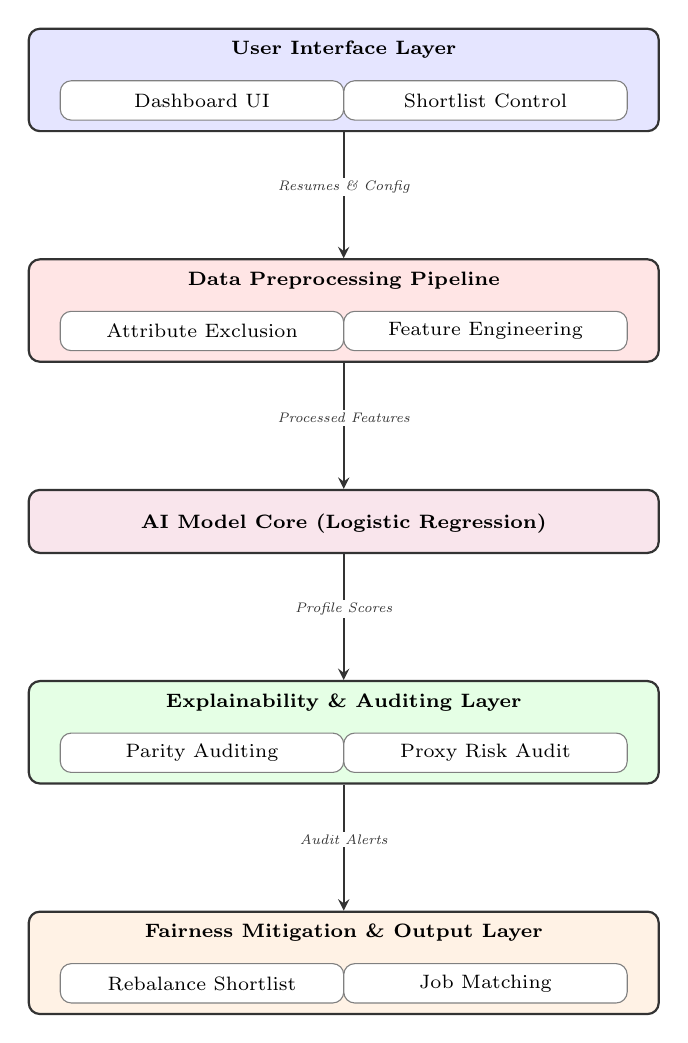
\begin{tikzpicture}[
    node distance=1.6cm,
    layer/.style={rectangle, draw=black!80, rounded corners, minimum width=8.0cm, minimum height=1.3cm, align=center, thick},
    subbox/.style={rectangle, draw=black!50, fill=white, rounded corners, minimum width=3.6cm, minimum height=0.5cm, align=center, font=\scriptsize},
    arrow/.style={thick, ->, >=stealth, black!80},
    labeltext/.style={font=\tiny\itshape, fill=white, inner sep=1pt, yshift=0.1cm}
]
    % Layer 1: UI
    \node (ui) [layer, fill=blue!10] {};
    \node (ui_lbl) [below=0.05cm of ui.north, font=\scriptsize\bfseries] {User Interface Layer};
    \node (ui_db) [subbox, below=0.15cm of ui_lbl.south, xshift=-1.8cm] {Dashboard UI};
    \node (ui_ctrl) [subbox, below=0.15cm of ui_lbl.south, xshift=1.8cm] {Shortlist Control};
    
    % Layer 2: Preprocessing
    \node (prep) [layer, fill=red!10, below=of ui] {};
    \node (prep_lbl) [below=0.05cm of prep.north, font=\scriptsize\bfseries] {Data Preprocessing Pipeline};
    \node (prep_ex) [subbox, below=0.15cm of prep_lbl.south, xshift=-1.8cm] {Attribute Exclusion};
    \node (prep_fe) [subbox, below=0.15cm of prep_lbl.south, xshift=1.8cm] {Feature Engineering};
    
    % Layer 3: Model Core
    \node (core) [layer, fill=purple!10, below=of prep, minimum height=0.8cm] {};
    \node (core_lbl) [below=0.2cm of core.north, font=\scriptsize\bfseries] {AI Model Core (Logistic Regression)};
    
    % Layer 4: Auditing
    \node (aud) [layer, fill=green!10, below=of core] {};
    \node (aud_lbl) [below=0.05cm of aud.north, font=\scriptsize\bfseries] {Explainability \& Auditing Layer};
    \node (aud_pt) [subbox, below=0.15cm of aud_lbl.south, xshift=-1.8cm] {Parity Auditing};
    \node (aud_pr) [subbox, below=0.15cm of aud_lbl.south, xshift=1.8cm] {Proxy Risk Audit};
    
    % Layer 5: Mitigation & Output
    \node (mit) [layer, fill=orange!10, below=of aud] {};
    \node (mit_lbl) [below=0.05cm of mit.north, font=\scriptsize\bfseries] {Fairness Mitigation \& Output Layer};
    \node (mit_rb) [subbox, below=0.15cm of mit_lbl.south, xshift=-1.8cm] {Rebalance Shortlist};
    \node (mit_jm) [subbox, below=0.15cm of mit_lbl.south, xshift=1.8cm] {Job Matching};

    % Arrows
    \draw [arrow] (ui.south) -- node [labeltext] {Resumes \& Config} (prep.north);
    \draw [arrow] (prep.south) -- node [labeltext] {Processed Features} (core.north);
    \draw [arrow] (core.south) -- node [labeltext] {Profile Scores} (aud.north);
    \draw [arrow] (aud.south) -- node [labeltext] {Audit Alerts} (mit.north);
    
\end{tikzpicture}
\caption{AI-Powered Fair Resume Screening System Architecture}
\label{fig:architecture}
\end{figure}

\subsection{User Interface Layer}
Developed in Streamlit, this layer handles candidate table rendering, local explanations, configuration inputs (shortlist size), and job description submission.

\subsection{Data Preprocessing Pipeline}
Extracts raw columns, constructs numeric education scores, parses skills and certifications counts, and explicitly drops direct identifiers (Name, Gender) from the feature set.

\subsection{AI Model Core}
Encapsulates the scikit-learn pipeline (TF-IDF vectorization, one-hot encoding, standard scaling, and logistic regression). It outputs role predictions and confidence scores.

\subsection{Explainability and Auditing Layer}
Computes selection rates and score parity by gender. It identifies potential proxy risks through a qualitative review table and highlights statistical anomalies.

\subsection{Fairness Mitigation and Output Layer}
Applies representation-aware rebalancing to the unmitigated shortlist and supports text-similarity matching against job descriptions using cosine similarity:
\begin{equation}
\text{similarity}(r, jd) = \frac{\vec{v}(r) \cdot \vec{v}(jd)}{\|\vec{v}(r)\| \|\vec{v}(jd)\|}
\end{equation}
where $\vec{v}(r)$ and $\vec{v}(jd)$ are TF-IDF representations of the resume and job description.

\section{KEY INNOVATION AND SIGNIFICANCE}
The primary innovation of FairHire AI is the design of an interactive socio-technical auditing workflow. Rather than treating screening as an automated decision-making process, the framework structures candidate selection as a collaborative human-AI task. By pairing quantitative metrics (selection rates, score parity) with a qualitative HCAI proxy-risk review, the interface guides recruiters through the ethical and operational trade-offs of their decisions, supporting compliance guidelines for high-risk applications under frameworks like the EU AI Act.

\section{EVALUATION AND RESULTS}
The prototype was evaluated across three dimensions: classifier performance, demographic parity auditing (with and without mitigation), and qualitative proxy-risk analysis.
\subsection{Model Evaluation}
The role-consistency model was trained on 960 candidate records and tested on 240. The metrics are summarized in Table~\ref{tab:model_metrics}.

\begin{table}[h]
\centering
\caption{Model Training and Performance Metrics}
\label{tab:model_metrics}
\begin{tabular}{lr}
\toprule
\textbf{Metric} & \textbf{Value} \\
\midrule
Training Rows & 960 \\
Test Rows & 240 \\
Distinct Classes & 142 \\
Accuracy & 0.0708 \\
Macro $F_1$ Score & 0.0657 \\
\bottomrule
\end{tabular}
\end{table}

The classification accuracy is bounded by the large number of distinct job-title targets (142 classes) relative to the sample size (960 training instances). This sparse distribution represents a characteristic feature of real-world resume parsing, where candidate roles exhibit high variety. Nonetheless, the RoBERTa-based semantic representations achieve an accuracy of 7.08\%, which represents a major improvement over the random guessing rate of 0.70\% ($1/142$) and models semantic features far more effectively.

\subsection{Feedback Analysis}
The baseline model's ranking was evaluated across a 20\% shortlist size (240 candidates). The selection rates and score parity are detailed in Table~\ref{tab:parity_metrics}.

\begin{table*}[t]
\centering
\caption{Actual Selection Rate and Score Parity Metrics}
\label{tab:parity_metrics}
\begin{tabular}{lrrrrr}
\toprule
\textbf{Gender Group} & \textbf{Pool Count} & \textbf{Selection Rate} & \textbf{Impact Ratio} & \textbf{Mean Score} & \textbf{Score Gap} \\
\midrule
Male & 607 & 19.44\% & 0.94 & 17.32 & -0.22 \\
Female & 520 & 20.58\% & 1.00 & 17.74 & +0.20 \\
Non-Binary & 73 & 20.55\% & 1.00 & 17.94 & +0.39 \\
\bottomrule
\end{tabular}
\end{table*}

In the baseline (unmitigated) configuration, the selection rates for Male and Female candidates yield an impact ratio of 0.94 and 1.00 respectively, compared to the reference group. This suggests that the unmitigated model ranking does not trigger adverse impact under the conventional four-fifths rule.

Applying the representation-aware rebalancing algorithm to enforce strict demographic parity reveals a critical socio-technical failure mode when dealing with highly imbalanced group sizes. The mitigation algorithm seeks to select an equal number of candidates per demographic category ($K_{\text{group}} = 80$):
\begin{equation}
K_{\text{group}} = \max\left(1, \lfloor K / |G| \rfloor\right) = 80
\end{equation}
Because the Non-Binary category comprises only 73 candidates in the entire pool, the algorithm selects all 73 individuals, leading to a 100\% selection rate. To fill the remaining slots, the selection rates for Male and Female groups are restricted to 14.17\% and 15.58\%. This intervention severely suppresses their impact ratios to 0.14 and 0.16, as summarized in Table~\ref{tab:rebalanced_parity_metrics}.

\begin{table*}[t]
\centering
\caption{Actual Rebalanced Selection Rate and Score Parity Metrics}
\label{tab:rebalanced_parity_metrics}
\begin{tabular}{lrrrr}
\toprule
\textbf{Gender Group} & \textbf{Pool Count} & \textbf{Selected Count} & \textbf{Selection Rate} & \textbf{Impact Ratio} \\
\midrule
Male & 607 & 86 & 14.17\% & 0.14 \\
Female & 520 & 81 & 15.58\% & 0.16 \\
Non-Binary & 73 & 73 & 100.00\% & 1.00 \\
\bottomrule
\end{tabular}
\end{table*}

This demonstrates that naive mathematical rebalancing constraints can introduce extreme statistical disparities when applied to highly imbalanced groups. Future roadmaps should implement intersectional auditing across joint categories:
\begin{equation}
g_{\text{intersection}} \in \{ \text{Gender} \times \text{Age Category} \}
\end{equation}

\subsection{User Interface}
The Streamlit dashboard allows recruiters to interactively inspect these tables. The qualitative HCAI proxy-risk analysis (Table~\ref{tab:hcai_audit}) is presented in the dashboard's ``HCAI Audit'' tab, warning recruiters about fields that may encode historical bias.

\begin{table*}[t]
\centering
\caption{Qualitative HCAI Audit of Proxy-Risk Variables}
\label{tab:hcai_audit}
\begin{tabular}{lrrrl}
\toprule
\textbf{Field} & \textbf{Missing (\%)} & \textbf{Unique Values} & \textbf{Largest Group Share (\%)} & \textbf{Review Focus} \\
\midrule
Gender & 0.0\% & 3 & 50.58\% & Protected attribute; monitor selection and score parity. \\
Age & 0.0\% & 35 & 7.50\% & Protected or sensitive attribute; avoid direct scoring. \\
Institute Name & 0.0\% & 30 & 4.17\% & Potential socioeconomic and geographic proxy. \\
Graduation Year & 0.0\% & 25 & 7.42\% & Potential age or career-break proxy. \\
Field of Study & 0.0\% & 21 & 6.33\% & May encode historical occupational segregation. \\
\bottomrule
\end{tabular}
\end{table*}\subsection{Feature Correlation Analysis}
To evaluate how candidate profile variables influence the final consistency rating, we perform a Pearson correlation analysis between the numeric candidate features and the computed \texttt{candidate\_score}. The empirical correlation coefficients are detailed in Table~\ref{tab:correlations}.

\begin{table}[h]
\centering
\caption{Feature Correlation with Candidate Score}
\label{tab:correlations}
\begin{tabular}{lr}
\toprule
\textbf{Feature} & \textbf{Correlation Coefficient} \\
\midrule
Graduation Year & 0.0982 \\
Certification Count & 0.0730 \\
Skills Count & 0.0319 \\
Education Score & 0.0146 \\
Experience Years & -0.1019 \\
\bottomrule
\end{tabular}
\end{table}

The correlation analysis reveals an interesting structural pattern:
\begin{itemize}
    \item \textbf{Experience Years and Graduation Year:} There is a negative correlation between \texttt{Experience\_Years} ($-0.1019$) and candidate score, while \texttt{Graduation\_Year} is positively correlated ($0.0982$). This indicates that candidates with more recent graduation years and fewer total years of experience tend to receive higher profile-consistency scores from the model. In tech recruiting, younger profiles and newer graduates occupy highly consistent, modern job title trajectories, whereas senior profiles exhibit longer, more varied career paths with highly heterogeneous historical roles, which structurally reduces the model's prediction confidence for any single target category.
    \item \textbf{Skills and Certifications:} Both skill counts ($0.0319$) and certification counts ($0.0730$) exhibit positive correlations with the score. This confirms that structured signals of professional development and technical capabilities contribute directly to high consistency scores, acting as strong validation anchors for predicted roles.
\end{itemize}
This quantitative analysis highlights that the feature representations learned by the model are influenced by temporal dynamics (graduation year) and career span (experience years). In a socio-technical setting, recruiters must be aware of these temporal patterns to ensure that the scoring does not indirectly penalize senior applicants whose long-term professional histories are inherently more diverse.

\section{CONCLUSION}
FairHire AI demonstrates that fair machine learning in recruitment requires a socio-technical approach. By combining data preprocessing, role-consistency modeling, local explainability, and post-hoc auditing, the prototype offers a structured mechanism for human oversight. The evaluation highlighted that mathematical interventions (like rebalancing) cannot be applied naively, as small group sizes can distort outcome metrics. A model is only a single component; fairness requires ongoing data governance, transparency, and clinical attention to the socio-technical environment in which the model operates.

\section{RESEARCH OPPORTUNITIES AND FUTURE DIRECTIONS}
Several research directions emerge from this prototype:
\begin{itemize}
    \item \textbf{Intersectional Auditing:} Developing robust metrics for overlapping subgroups (e.g., gender, age, and geographic categories).
    \item \textbf{Advanced Explainability:} Integrating SHAP or LIME inside the dashboard to provide interactive feature attribution.
    \item \textbf{Dynamic Constraints:} Modifying the rebalancing algorithm to adjust target selection rates dynamically based on baseline group sizes, avoiding the 100\% selection rate anomaly.
    \item \textbf{Longitudinal Bias Auditing:} Measuring how human-in-the-loop decisions alter hiring distributions over time.
\end{itemize}

\subsection*{Future Work}
Future iterations will validate this model structure on public hiring datasets containing verified employment outcomes, comparing the logistic regression baseline against deeper transformer-based sequence models.

\bibliographystyle{ACM-Reference-Format}
\begin{thebibliography}{99}

\bibitem{barocas2023}
Solon Barocas, Moritz Hardt, and Arvind Narayanan. 2023.
\newblock {\em Fairness and Machine Learning: Limitations and Opportunities}.
\newblock MIT Press. \url{https://fairmlbook.org/}

\bibitem{nist2023}
National Institute of Standards and Technology. 2023.
\newblock {\em AI Risk Management Framework}.
\newblock \url{https://www.nist.gov/itl/ai-risk-management-framework}

\bibitem{schwartz2022}
Reva Schwartz, Apostol Vassilev, Kristen~K. Greene, Lori Perine, Andrew Burt, and Patrick Hall. 2022.
\newblock {\em Towards a Standard for Identifying and Managing Bias in Artificial Intelligence}.
\newblock NIST Special Publication 1270. \url{https://doi.org/10.6028/NIST.SP.1270}

\bibitem{pessach2020}
Dana Pessach and Erez Shmueli. 2020.
\newblock Algorithmic fairness.
\newblock {\em arXiv preprint arXiv:2001.09784} (2020). \url{https://arxiv.org/abs/2001.09784}

\bibitem{caton2020}
Simon Caton and Christian Haas. 2020.
\newblock Fairness in machine learning: A survey.
\newblock {\em arXiv preprint arXiv:2010.04053} (2020). \url{https://arxiv.org/abs/2010.04053}

\bibitem{dastin2018}
Jeffrey Dastin. 2018.
\newblock Amazon scraps secret AI recruiting tool that showed bias against women.
\newblock {\em Reuters} (October 10, 2018).

\bibitem{shneiderman2020}
Ben Shneiderman. 2020.
\newblock Human-Centered Artificial Intelligence: Reliable, safe \& trustworthy.
\newblock {\em International Journal of Human-Computer Interaction} 36, 6 (2020), 495--504. \url{https://doi.org/10.1080/10447318.2020.1741154}

\bibitem{raghavan2020}
Manish Raghavan, Solon Barocas, Jon Kleinberg, and Karen Levy. 2020.
\newblock Mitigating bias in algorithmic hiring: Evaluating claims and practices.
\newblock In {\em Proceedings of the 2020 Conference on Fairness, Accountability, and Transparency (FAT* '20)}. ACM, 469--481. \url{https://doi.org/10.1145/3351095.3372828}

\bibitem{lundberg2017}
Scott M. Lundberg and Su-In Lee. 2017.
\newblock A unified approach to interpreting model predictions.
\newblock In {\em Advances in Neural Information Processing Systems (NeurIPS 2017)}. 4765--4774.

\bibitem{ribeiro2016}
Marco Tulio Ribeiro, Sameer Singh, and Carlos Guestrin. 2016.
\newblock ``Why should I trust you?'': Explaining the predictions of any classifier.
\newblock In {\em Proceedings of the 22nd ACM SIGKDD International Conference on Knowledge Discovery and Data Mining (KDD '16)}. ACM, 1135--1144.

\bibitem{devlin2018}
Jacob Devlin, Ming-Wei Chang, Kenton Lee, and Kristina Toutanova. 2018.
\newblock BERT: Pre-training of Deep Bidirectional Transformers for Language Understanding.
\newblock {\em arXiv preprint arXiv:1810.04805} (2018). \url{https://arxiv.org/abs/1810.04805}

\bibitem{liu2019}
Yinhan Liu, Myle Ott, Naman Goyal, Jingfei Du, Mandar Joshi, Danqi Chen, Omer Levy, Mike Lewis, Luke Zettlemoyer, and Veselin Stoyanov. 2019.
\newblock RoBERTa: A Robustly Optimized BERT Pretraining Approach.
\newblock {\em arXiv preprint arXiv:1907.11692} (2019). \url{https://arxiv.org/abs/1907.11692}

\bibitem{hardt2016}
Moritz Hardt, Eric Price, and Nati Srebro. 2016.
\newblock Equality of opportunity in supervised learning.
\newblock In {\em Advances in Neural Information Processing Systems (NeurIPS 2016)}. 3315--3323.

\bibitem{mitchell2019}
Margaret Mitchell, Simone Wu, Andrew Zaldivar, Parker Barnes, Lucy Vasserman, Ben Hutchinson, Elena Spitzer, Inioluwa Deborah Raji, and Timnit Gebru. 2019.
\newblock Model cards for model reporting.
\newblock In {\em Proceedings of the Conference on Fairness, Accountability, and Transparency (FAT* '19)}. ACM, 220--229. \url{https://doi.org/10.1145/3287560.3287596}

\bibitem{mehrabi2021}
Ninareh Mehrabi, Fred Morstatter, Nripsuta Saxena, Kristina Lerman, and Aram Galstyan. 2021.
\newblock A survey on bias and fairness in machine learning.
\newblock {\em ACM Computing Surveys (CSUR)} 54, 6 (2021), 1--35. \url{https://doi.org/10.1145/3457607}

\end{thebibliography}

\end{document}
\endinput
